\documentclass[11pt]{article}
\usepackage[utf8]{inputenc}
\usepackage[T1]{fontenc}
\usepackage{graphicx}
\usepackage{amsmath}
\title{TP 1}
\author{Jouve Vincent 3671083 Lenoir Romain 3670199}
\date{}
\graphicspath{ {./} }

\begin{document} 
\maketitle 

\part*{\Large Partie 1}
\section*{\large Question 1}
$M_x$ et $M_y$ sont séparable, si on prend en compte le facteur $\frac{1}{4}$ avec $h_y = \begin{pmatrix}0.5\\1\\0.5\end{pmatrix}$
et $h_x = \begin{pmatrix}-0.5\\0\\0.5\end{pmatrix}$ on a que $M_x = h_y \times h_x^\top$ et $M_y = h_x \times h_y^\top$

\section*{\large Question 2}
On gagne en complexité. on passe de 9 à 6 opérations pour un filtre 3x3.

\section*{\large Question 3}
En appliquant un masque gaussien sur les normes des gradients on fait en sorte que ce qui se passe au centre du patch est plus important que ce qui se passe plus loin sur les côtés. Au final le SIFT exprimera plus fortement ce qu'il se passe au centre du patch.

\section*{\large Question 4}
Le SIFT est une façon de représenter un patch, il donne de l'information. La discrétisation permet par la suite de compresser l'information d'un patch avec l'histogramme, on passe de deux matrices de 16*16 à un vecteur de taille 128. Un même SIFT peut être calculé grâce à deux patchs proches mais pas identique. On a donc compressé et généraliser l'information sans trop en perdre.

\section*{\large Question 5}
Pour la 1ère étape on regarde si la norme est en-dessous d'un seuil, si oui on fixe le descripteur au vecteur nul. Ce sont des descripteurs portant quasiment aucune information et probablement que du bruit, c'est pour cela qu'on le fixe au descripteur nul.
\hfill \break 
Pour la seconde étape on normalise le descripteur, on aura donc le même ordre de grandeur pour toutes les composantes de tous les descripteurs. Cela permet d’être robuste à la luminosité de l'image, et de ne pas éloigné deux patch qui présenterai la même forme mais l'un moins lumineux que l'autre.
\hfill \break 
Pour la dernière étape les valeurs des composantes sont seuillées, car on ne veut pas qu'une direction l'importe et soit la seule représentante du patch, auquel cas on pourrait avoir du mal à différencier deux SIFT juste en se basant sur le fait qu'ils aient la même composante principale, ils seraient trop proche géométriquement parlant, et le reste ne compterai pas assez pour les différencier.


\section*{\large Question 6}
ça permet de comparer les patchs entre eux. On généralise un peu mais pas trop, on garde suffisamment d'informations sur les directions et les normes pour décrire le patch tout en généralisant.

\section*{\large Question 7}

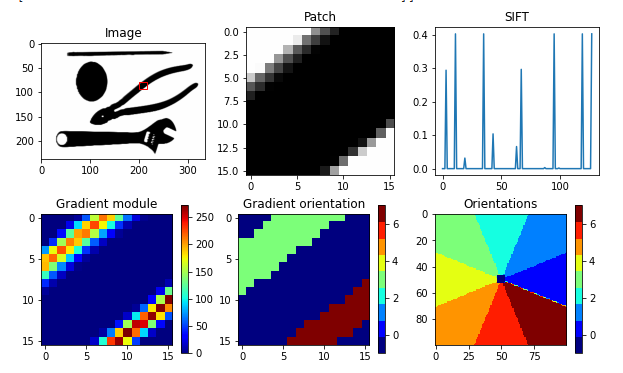
\includegraphics{q7}
Les orientations des gradients vont bien du noir vers le blanc. De même les normes des gradients sont d'autant plus grandes qu'elles sont sur une frontière noir blanc. 

\part*{\Large Partie 2}
\section*{\large Question 8}
Le but est de décrire le contenu de l’image comparée, pour cela il faut une description commune. Nous pourrons ensuite comparer le nombre de sift qui appartiennent à chaque cluster. Deux images ayant un nombre de sift identique pour chaque cluster sera probablement assez similaire.

\section*{\large Question 9}
Pour trouver le minimum il suffit de trouver où la dérivé s'annule. \\
\begin{align*}
2*\sum_{i=1}^{n} \vec{x_i}-\vec{c} = 0 &\iff \sum_{i=1}^{n} \vec{x_i} - \sum_{i=1}^{n} \vec{c} = 0 \\
&\iff \sum_{i=1}^{n}\vec{x_i} - n*\vec{c} = 0\\
&\iff \vec{c} = \frac{1}{n}\sum_{i=1}^{n} \vec{x_i}
\end{align*}
\\
Le c qui minimise l'équation est bien le barycentre.

\section*{\large Question 10}
Soit on a une idée du nombre qu'il nous faut, imaginons qu’on veuille différencier 4 classes de patch, on aura alors besoin de 4 clusters. Sinon on test pour pleins de K et à l'aide d’indice comme l’indice de dunn et/ou xie-beni qui donne une indication sur la qualité des clusters, on choisit le meilleur nombre de cluster.

\section*{\large Question 11}
Pour généraliser et ainsi être robuste aux changements comme la luminosité ou les translations. 

\section*{\large Question 12}
Parmi les clusters on peut trouver ce genre de chose, qui représente les 50 régions d'images les plus proche du représentant du cluster.

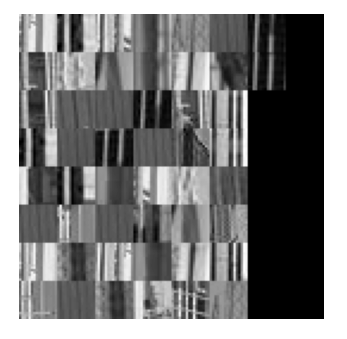
\includegraphics{q12_1}

Ici on voit que pour ce cluster cela fonctionne plutôt bien, on a bien regroupé les régions qui présentent deux barres parallèles. Pour certaines régions on peut même y voir des barreaux.

\part*{\Large Partie 3}
\section*{\large Question 13}
Chaque composante i de z représente le nombre de fois que le SIFT-type i est le plus proche d'un SIFT correspondant à un patch de l'image.
\section*{\large Question 14}
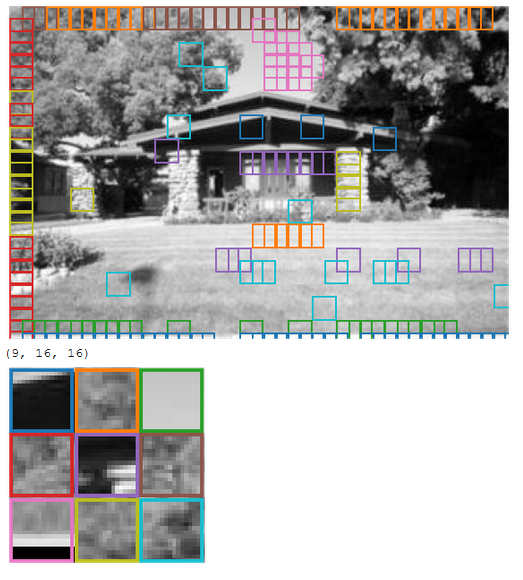
\includegraphics[height=15cm]{q14}
Ici on peut voir visuellement les 9 SIFT-type les plus présent dans l'image et on voit même où est-ce qu'ils sont présents. On voit que certain SIFT-type représentant le bord des fenêtres, ils sont assez nombreux(en violet). Ce qui est pas mal pour classifier ensuite cette image comme une maison, puisque toutes les maisons vont avoir beaucoup de ce SIFT-type. 
\section*{\large Question 15}
Il permet d'unifier les données, que chaque patch soit représenté par les mêmes caractéristiques. Ici le codage correspond à un vecteur nul de taille k (k étant aussi la taille du dictionnaire) avec un 1 sur l'élément qui correspond au SIFT-type le plus proche du SIFT calculer à partir du patch. On pourrait utiliser un codage à n plus proches voisins, ce qui donnerai un vecteur nul de taille k avec un 1 sur les éléments correspondant aux n SIFT-type les plus proches. Ce qui permet d'avoir une description plus ample des images. 

\section*{\large Question 16}
On cherche à avoir une description de l'image de façon. Ici on a découpé l'image en patch qu'on a encodé, il faut maintenant les agrégés pour avoir un vecteur caractérisant l'image entière, c'est à ça que sert le polling. On pourrait utiliser un polling tf-idf qui ferait ressortir les SIFT les moins observé parmi toutes les images, et donc ferait ressortir les spécificités des images.

\section*{\large Question 17}
L'intérêt de normaliser est d'avoir toutes les composant du vecteur z à la même échelle. Il pourrait y avoir une trop grande différence du fait que les images ne sont pas toutes de la même taille et donc elles n'auraient pas toutes le même nombre de patchs et des échelles bien différente. ça simplifira l'optimisation des modèle d'apprentissage. On pourrait utiliser la normalisation L1. 

\part*{\Large TP 3}
\section*{\large Question 1}
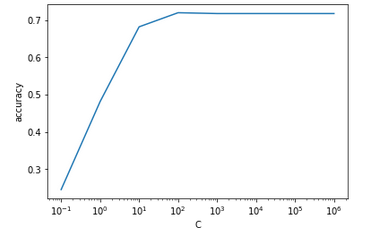
\includegraphics{q2}

Pour C=0.1 le modèle est trop complexe, les poids sont trop grand, et la généralisation est mauvaise. On a une accuracy de 0.24.
Après l'accuracy monte est atteint sont maximum pour c=100, soit 0.72. Le modèle est plus simple et généralise mieux.
\section*{\large Question 2}
C est le paramètre de poids de la régularisation, c'est-à-dire plus C est grand plus la régularisation sera forte dans la loss.
Le paramètre kernel représente le type de modèle utilisé, soit un modèle linéaire ou polynomial ou d'autre encore. Dans le cas du polynôme il existe un paramètre degré qui est le degré du polynôme.

\section*{\large Question 3}
Il faut tester le modèle sur un set qui n'a pas permis d'apprendre le modèle(apprentissage des hyper-paramètres compris). Autrement dit un set que le modèle n'a jamais vu auparavant, pour ne pas avoir une mesure biaisé par l'apprentissage. 

\end{document}
